\documentclass[10pt,aspectratio=169]{beamer}
\usepackage[T1]{fontenc}
\usepackage[utf8]{inputenc}
\usepackage[vietnamese]{babel}
\usepackage{graphicx}
\usepackage{amsmath}
\usepackage{booktabs}
\usepackage{multicol}
\usepackage{caption}
\usepackage{tikz}
\usetikzlibrary{shapes.geometric, arrows.meta, positioning, calc, scopes}

\setbeamertemplate{caption}[numbered]
\captionsetup[figure]{font=scriptsize, textfont=it, labelfont=bf}

\graphicspath{{../Images/}}

% --- Custom Colors HCMUT ---
\definecolor{hcmutblue}{HTML}{003A70}
\definecolor{hcmutred}{HTML}{A8192E}
\definecolor{lightgray}{HTML}{F4F4F4}
\definecolor{darktext}{HTML}{2D3436}

% --- Theme Settings ---
\mode<presentation> {
    \usetheme{Madrid}
    
    % Color theme overrides
    \setbeamercolor{palette primary}{bg=hcmutblue,fg=white}
    \setbeamercolor{palette secondary}{bg=hcmutblue!80!black,fg=white}
    \setbeamercolor{palette tertiary}{bg=hcmutred,fg=white}
    \setbeamercolor{palette quaternary}{bg=black,fg=white}
    \setbeamercolor{structure}{fg=hcmutblue}
    \setbeamercolor{section in toc}{fg=darktext}
    \setbeamercolor{frametitle}{bg=hcmutblue,fg=white}
    \setbeamercolor{title}{bg=hcmutblue,fg=white}
    \setbeamercolor{block title}{bg=hcmutblue,fg=white}
    \setbeamercolor{block body}{bg=lightgray,fg=darktext}
    
    % Minimal settings
    \setbeamertemplate{navigation symbols}{}
    \setbeamertemplate{items}[circle]
    \setbeamerfont{frametitle}{size=\Large, series=\bfseries}
    
    % Custom footline to show section and subsection (and remove date)
    \setbeamertemplate{footline}
    {
      \leavevmode%
      \hbox{%
      \begin{beamercolorbox}[wd=.333333\paperwidth,ht=2.25ex,dp=1ex,center]{author in head/foot}%
        \usebeamerfont{author in head/foot}\insertsectionhead
      \end{beamercolorbox}%
      \begin{beamercolorbox}[wd=.333333\paperwidth,ht=2.25ex,dp=1ex,center]{title in head/foot}%
        \usebeamerfont{title in head/foot}\insertsubsectionhead
      \end{beamercolorbox}%
      \begin{beamercolorbox}[wd=.333333\paperwidth,ht=2.25ex,dp=1ex,right]{date in head/foot}%
        \usebeamerfont{date in head/foot}\hspace*{2em}
        \insertframenumber{} / \inserttotalframenumber\hspace*{2ex} 
      \end{beamercolorbox}}%
      \vskip0pt%
    }
}

% Thiết lập title
\title[]{THIẾT KẾ, MÔ PHỎNG VÀ THI CÔNG HỆ THỐNG TẠO DÁNG ĐI THÍCH NGHI VÀ ỔN ĐỊNH TƯ THẾ CHO ROBOT BỐN CHÂN SỬ DỤNG PHẢN HỒI IMU}
\author[]{Sinh viên thực hiện:\\ Trương Tuấn An (2210041)\\ Võ Quế Long (2211910)\\ \vspace{0.3cm} Giảng viên hướng dẫn:\\ TS. Nguyễn Lê Dũng}
\institute{}
\date{}

\begin{document}

\begin{frame}[plain]
    \begin{tikzpicture}[remember picture,overlay]
        % Top banner background (Navy Blue)
        \fill[hcmutblue] (current page.north west) rectangle ([yshift=-4.5cm]current page.north east);
        % Crimson Red accent line
        \fill[hcmutred] ([yshift=-4.5cm]current page.north west) rectangle ([yshift=-4.65cm]current page.north east);
        
        % Logo placement (Top Right)
        \node[anchor=north east, inner sep=0.7cm] at (current page.north east) {
\includegraphics[width=2.5cm]{../presentation/reference/images/hcmut_logo_transparent.png}};
        
        % Main Title
        \node[anchor=west, text=white, font=\Large\bfseries, text width=12cm] at ([xshift=1cm, yshift=-2cm]current page.north west) {THIẾT KẾ, MÔ PHỎNG VÀ THI CÔNG\\ \textcolor{hcmutred}{HỆ THỐNG TẠO DÁNG ĐI THÍCH NGHI}};
        % Subtitle
        \node[anchor=west, text=lightgray, font=\normalsize, text width=12cm] at ([xshift=1cm, yshift=-3.3cm]current page.north west) {VÀ ỔN ĐỊNH TƯ THẾ CHO ROBOT BỐN CHÂN\\SỬ DỤNG PHẢN HỒI IMU};
        
        % Group Info & Details
        \node[anchor=north west, text=hcmutblue, font=\Large\bfseries] at ([xshift=1cm, yshift=-5.5cm]current page.north west) {NHÓM THỰC HIỆN:};
        \node[anchor=north west, text=darktext, font=\normalsize] at ([xshift=1cm, yshift=-6.4cm]current page.north west) {\textbf{SVTH:} Trương Tuấn An (2210041) - Võ Quế Long (2211910)};
        \node[anchor=north west, text=darktext, font=\normalsize] at ([xshift=1cm, yshift=-7.1cm]current page.north west) {\textbf{GVHD:} TS. Nguyễn Lê Dũng};
        
        % Aesthetic watermark
        \fill[hcmutred!80] (current page.south east) -- ([yshift=1.5cm]current page.south east) -- ([xshift=-1.5cm]current page.south east) -- cycle;
    \end{tikzpicture}
\end{frame}

\begin{frame}{Nội dung trình bày}
  \tableofcontents[hideallsubsections]
\end{frame}

\AtBeginSection[]
{
  \begin{frame}{Nội dung trình bày}
    \tableofcontents[currentsection, hideallsubsections]
  \end{frame}
}

% --------------------------------------------------
\section{Giới thiệu}
% --------------------------------------------------

\begin{frame}{Đặt vấn đề}
  \begin{itemize}
      \item \textbf{Thực tiễn:} Robot có chân linh hoạt trong môi trường gồ ghề hơn so với bánh xe hoặc bánh xích.
      \item \textbf{Thách thức:} Đòi hỏi khả năng giữ thăng bằng cao và hệ thống điều khiển phức tạp.
      \item \textbf{Giải pháp:} Thiết kế chế tạo nguyên mẫu robot bốn chân 12 DOF cỡ nhỏ. Tối ưu bộ điều khiển cân bằng sử dụng IMU trên môi trường phân tán ROS 2.
  \end{itemize}
\end{frame}

\begin{frame}{Mục tiêu đề tài}
  \begin{enumerate}
      \item \textbf{Cơ khí \& Động học:} Thiết kế 3D, thi công khung robot, xây dựng mô hình IK cho cơ cấu 3 DOF.
      \item \textbf{Quy hoạch quỹ đạo:} Nội suy đa thức quỹ đạo chân hình chữ D liên tục trơn tru.
      \item \textbf{Điều khiển ổn định:} Bộ điều khiển PID thích nghi với hai chế độ tĩnh (HOME) và động (GAIT).
      \item \textbf{Phần mềm:} Xây dựng kiến trúc điều khiển trên ROS 2, liên kết Gazebo.
  \end{enumerate}
\end{frame}

% --------------------------------------------------
\section{Lý thuyết động học và quy hoạch dáng đi}
% --------------------------------------------------

\begin{frame}{Mô hình động học nghịch (IK)}
  \begin{columns}
      \begin{column}{0.5\textwidth}
          \begin{itemize}
              \item Sử dụng phương pháp hình học giải tích cho cấu trúc 3-DOF: Coxa, Femur, Tibia.
              \item Cho phép nội suy tọa độ không gian làm việc Cartesian $(x,y,z)$ thành các góc khớp $(\theta_1, \theta_2, \theta_3)$ với tốc độ cao, phục vụ thời gian thực.
          \end{itemize}
      \end{column}
      \begin{column}{0.5\textwidth}
          \begin{figure}
              \centering
              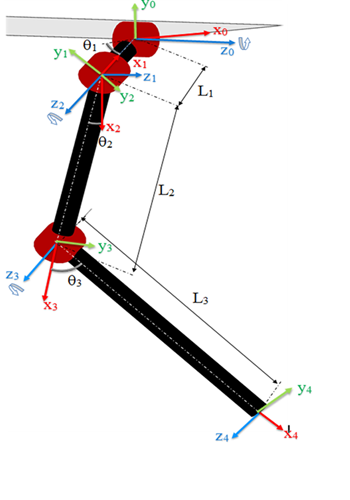
\includegraphics[width=0.8\linewidth, height=0.7\textheight, keepaspectratio]{kinematics/single_leg_3dof.png}
              \caption{Mô hình hình học giải IK một chân}
          \end{figure}
      \end{column}
  \end{columns}
\end{frame}

\begin{frame}{Dáng đi chéo góc (Trot Gait)}
  \begin{columns}
      \begin{column}{0.4\textwidth}
          \begin{itemize}
              \item \textbf{Dáng đi Trot:} Hai chân đối chéo (Ví dụ: Trái-Trước và Phải-Sau) cùng vung, hai chân còn lại cùng chống.
              \item Đảm bảo luôn có 2 chân tiếp đất, tối ưu hóa sự cân bằng động.
          \end{itemize}
      \end{column}
      \begin{column}{0.6\textwidth}
          \begin{figure}
              \centering
              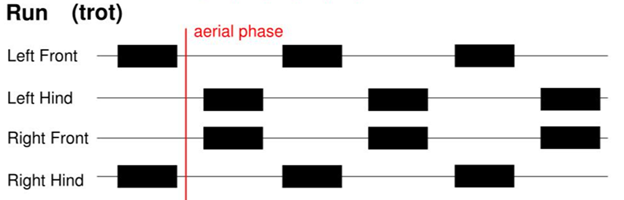
\includegraphics[width=\linewidth, height=0.7\textheight, keepaspectratio]{gait_planner/trot_gait_table.png}
              \caption{Bảng phân bổ thời gian pha Trot}
          \end{figure}
      \end{column}
  \end{columns}
\end{frame}

\begin{frame}{So sánh quy hoạch Đa thức (Cubic vs Quintic)}
  \begin{columns}
      \begin{column}{0.4\textwidth}
          \begin{itemize}
              \item Thay vì đa thức bậc 3 (Cubic), hệ thống sử dụng \textbf{Đa thức bậc 5 (Quintic)}.
              \item Triệt tiêu vô hạn gia tốc tại các điểm nhấc/hạ chân ($\ddot{s} = 0$).
              \item Giảm sốc cơ học, bảo vệ hệ thống truyền động.
          \end{itemize}
      \end{column}
      \begin{column}{0.6\textwidth}
          \begin{figure}
              \centering
              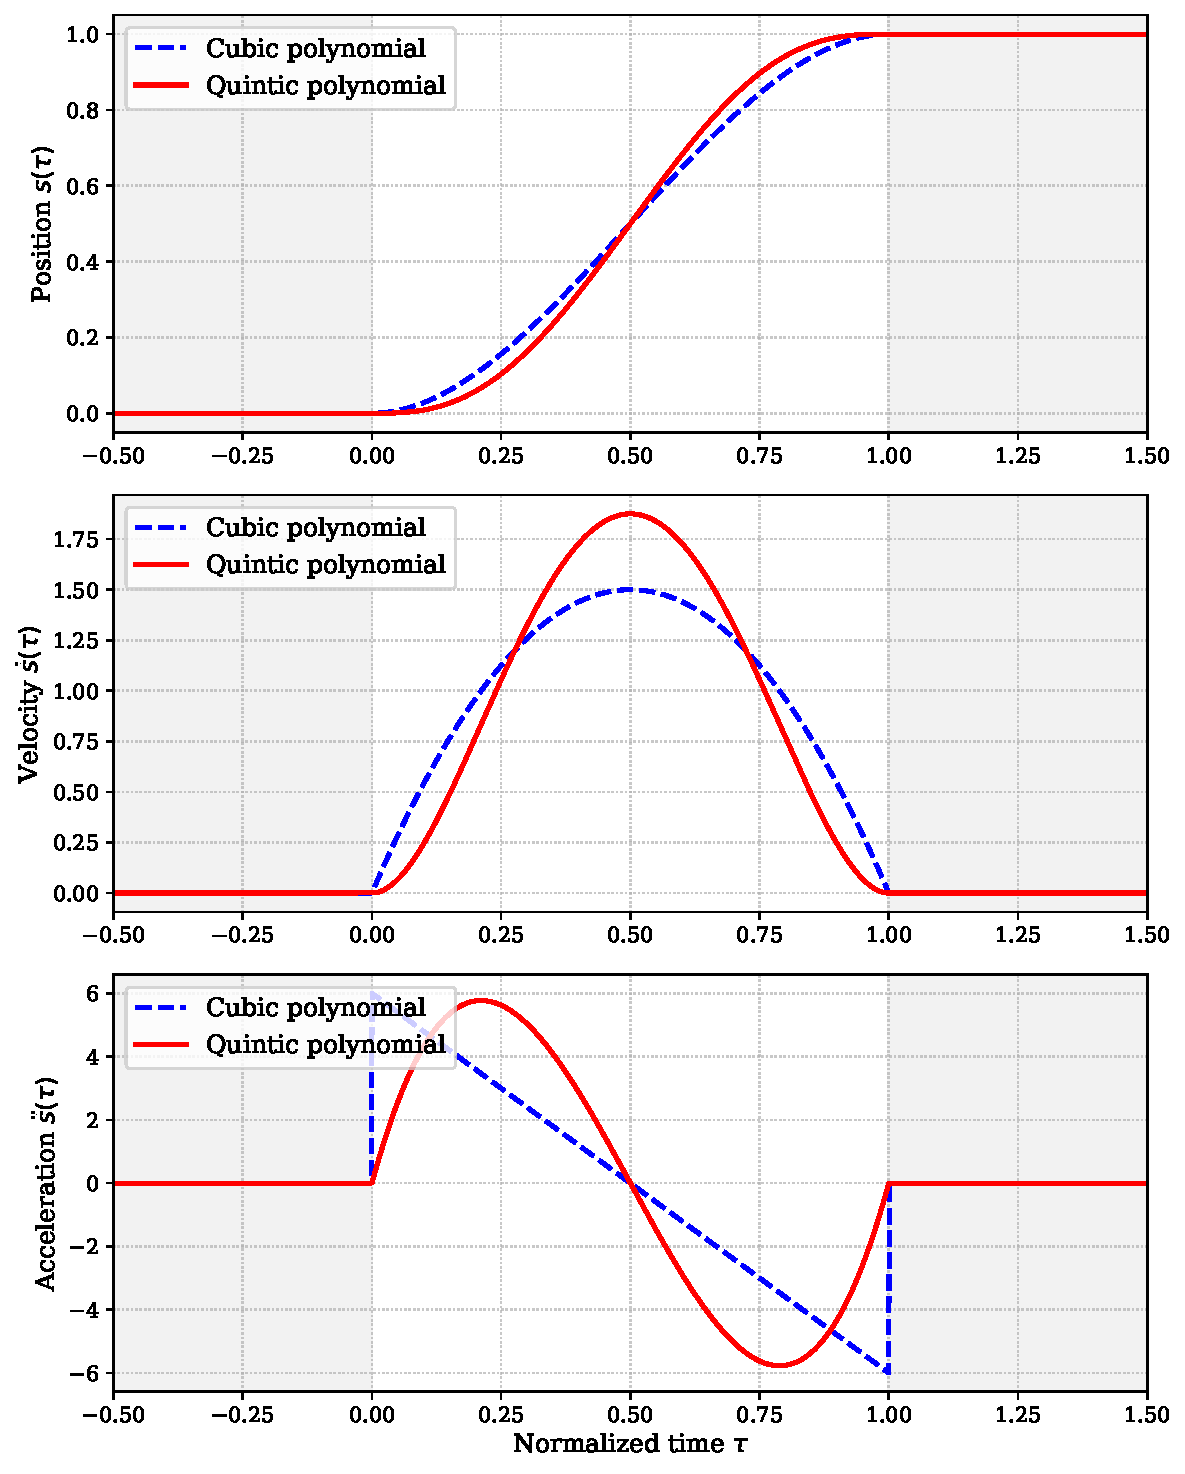
\includegraphics[height=0.7\textheight, keepaspectratio]{gait_planner/cubic_vs_quintic.pdf}
              \caption{So sánh gia tốc giữa Cubic và Quintic}
          \end{figure}
      \end{column}
  \end{columns}
\end{frame}


% --------------------------------------------------
\section{Thiết kế và thực hiện phần cứng}
% --------------------------------------------------

\begin{frame}{Thiết kế cơ khí}
  \begin{columns}
      \begin{column}{0.5\textwidth}
          \begin{itemize}
              \item Khung thân và các khớp chân được thiết kế trên SolidWorks.
              \item Vật liệu chế tạo: Nhựa in 3D PLA kết hợp với các vòng bi gia cố tại khớp vai.
              \item Động cơ: 12 Bus Servo ST3215.
          \end{itemize}
      \end{column}
      \begin{column}{0.5\textwidth}
          \begin{figure}
              \centering
              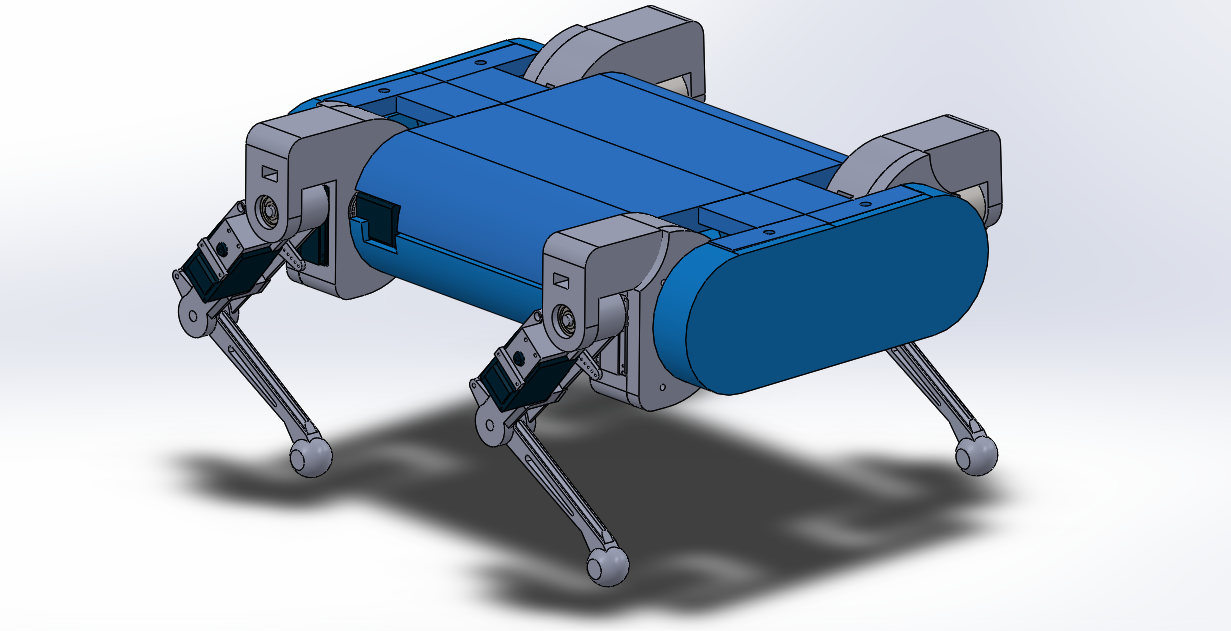
\includegraphics[width=0.8\linewidth, height=0.7\textheight, keepaspectratio]{hardware/preview_design.png}
              \caption{Bản thiết kế 3D của nguyên mẫu robot}
          \end{figure}
      \end{column}
  \end{columns}
\end{frame}

\begin{frame}{Thiết kế mạch nhúng và cảm biến}
  \begin{columns}
      \begin{column}{0.4\textwidth}
          \begin{itemize}
              \item \textbf{Máy tính nhúng:} NVIDIA Jetson Nano.
              \item \textbf{Cảm biến:} BNO055 IMU (I2C).
              \item \textbf{Giao tiếp servo:} Chia 2 nhánh Serial bằng mạch Bus Servo Adapter để giảm tải UART.
          \end{itemize}
      \end{column}
      \begin{column}{0.6\textwidth}
          \begin{figure}
              \centering
              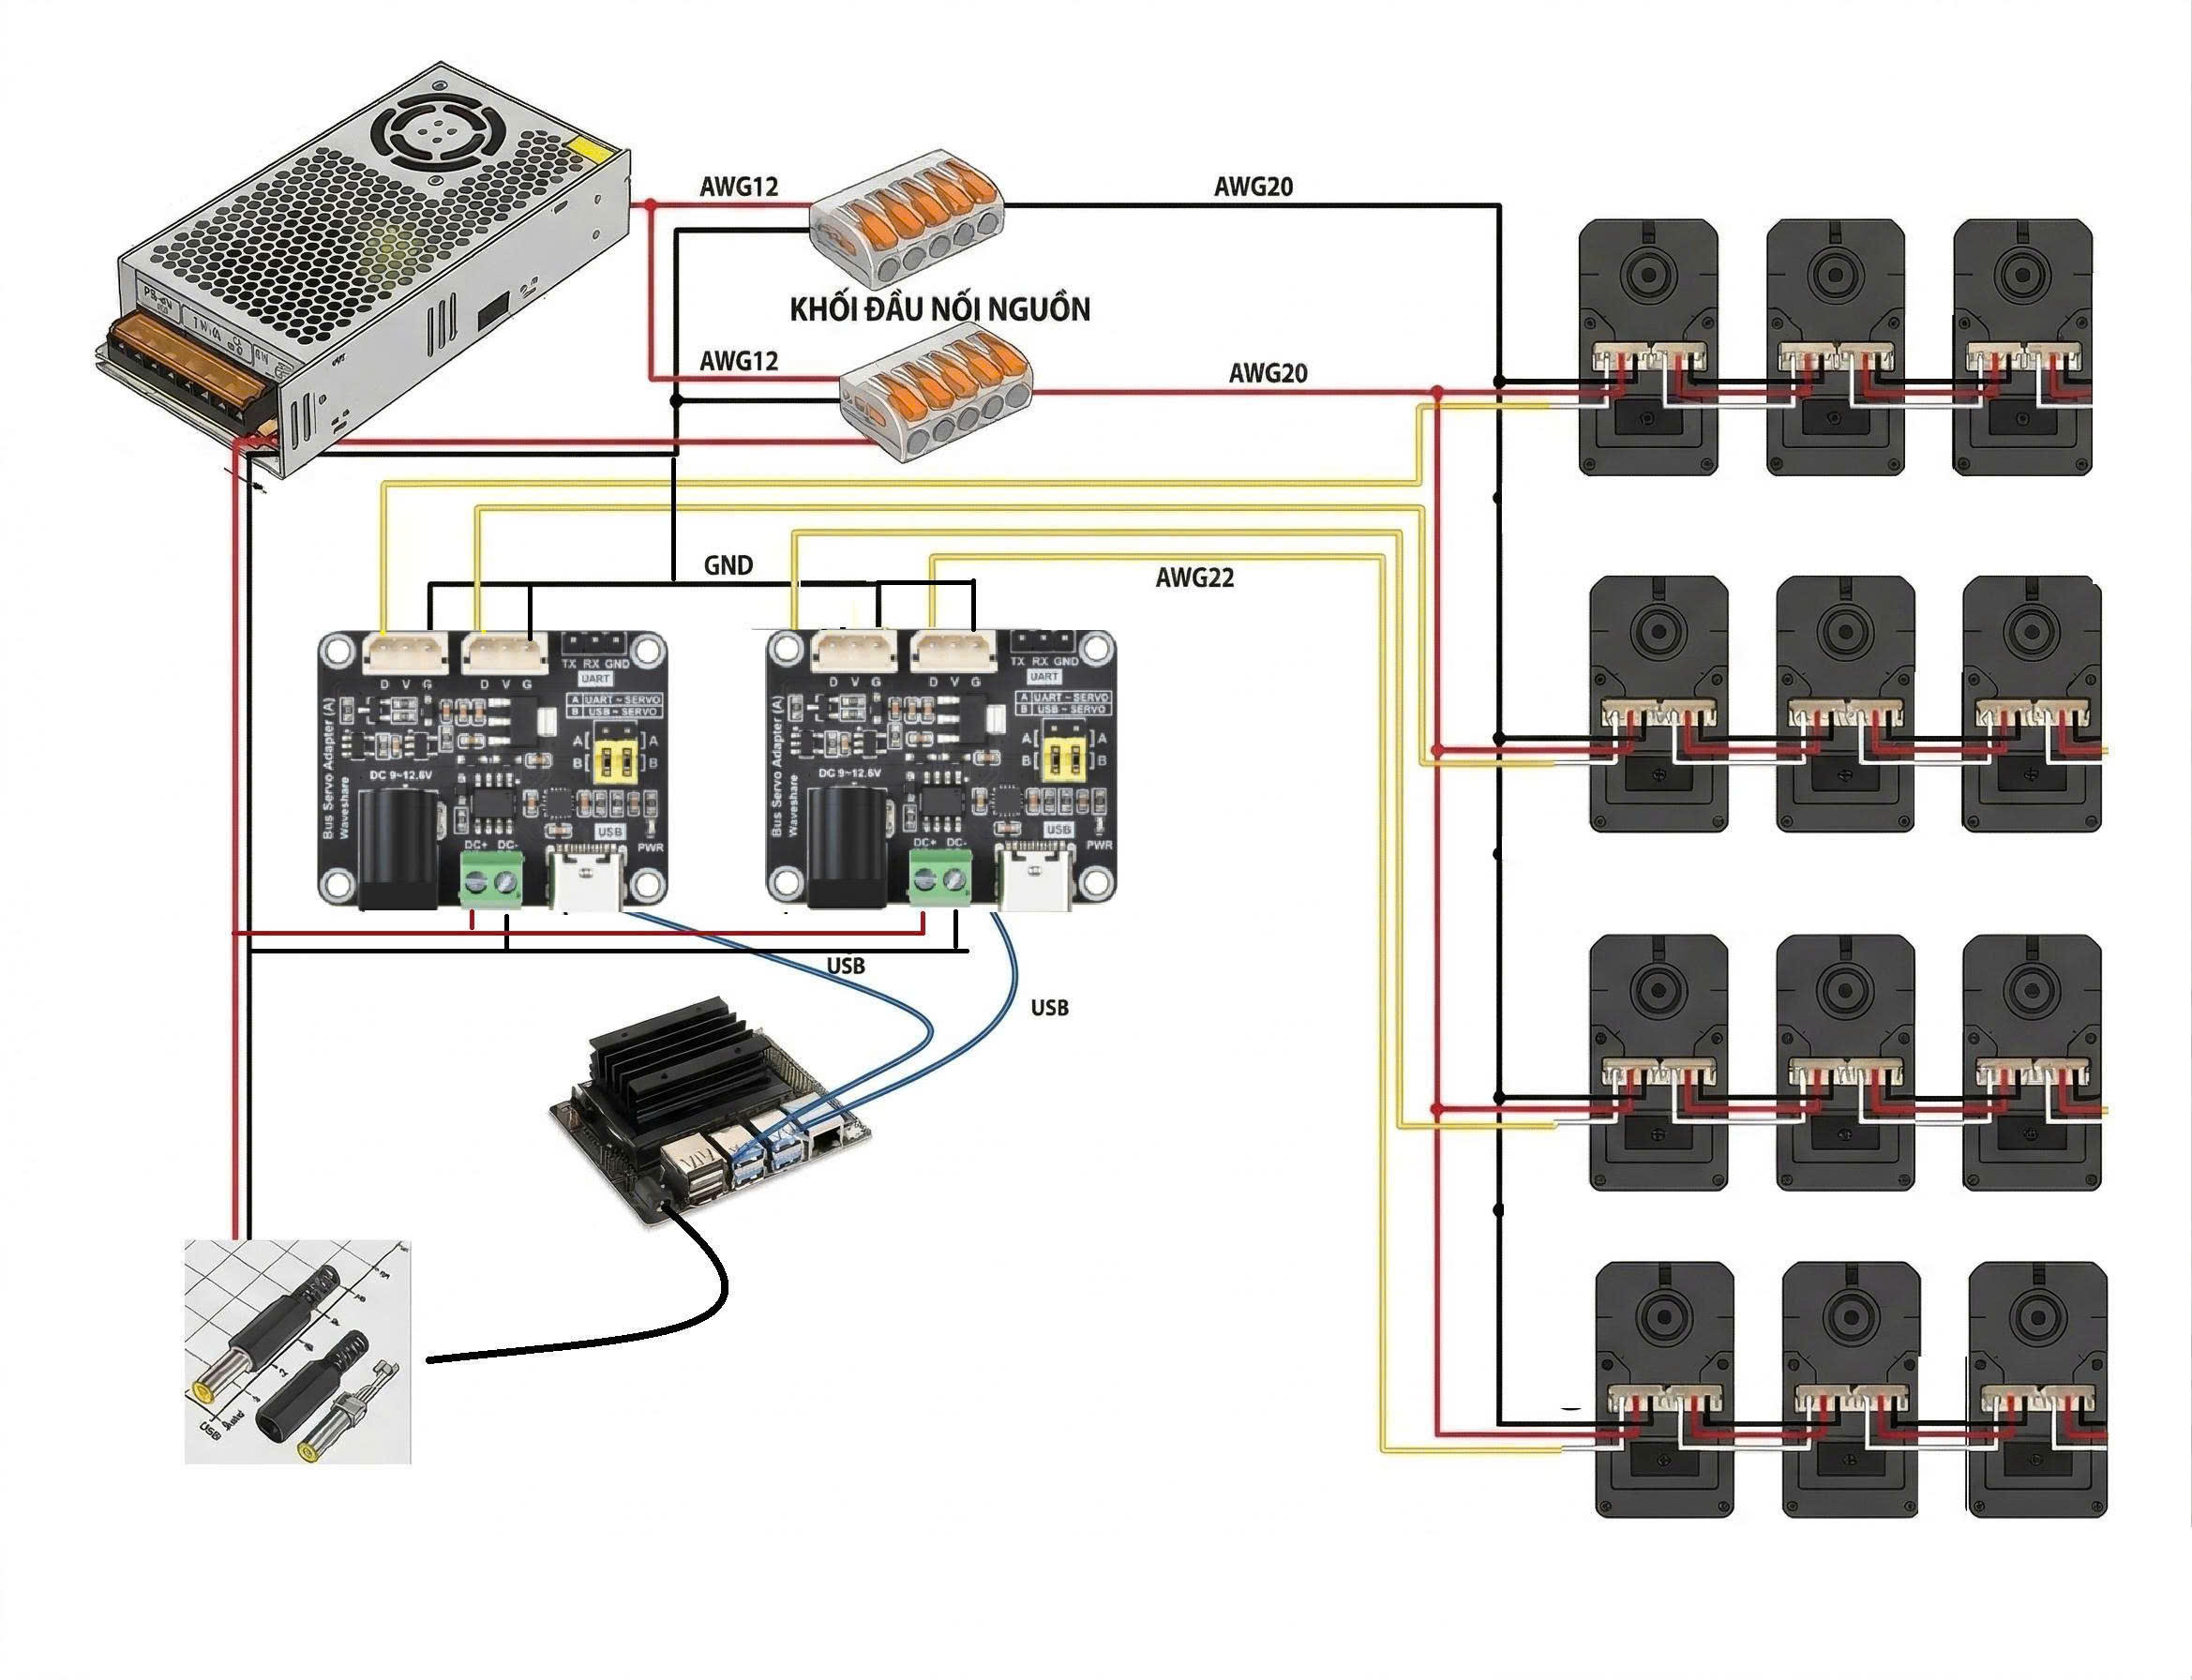
\includegraphics[width=\linewidth, height=0.7\textheight, keepaspectratio]{hardware/system_wiring_diagram.jpg}
              \caption{Sơ đồ hệ thống dây điện tổng thể}
          \end{figure}
      \end{column}
  \end{columns}
\end{frame}

\begin{frame}{Robot thực tế hoàn thiện}
  \begin{columns}
      \begin{column}{0.5\textwidth}
          \begin{itemize}
              \item Trọng lượng: $\approx 3.5$ kg.
              \item Hoàn thiện lắp ráp cơ khí và tinh chỉnh hệ thống điện.
              \item Cấu trúc chân: Nối tiếp (Serial) với cấu hình Full-Elbow (Khủy gập trong).
          \end{itemize}
      \end{column}
      \begin{column}{0.5\textwidth}
          \begin{figure}
              \centering
              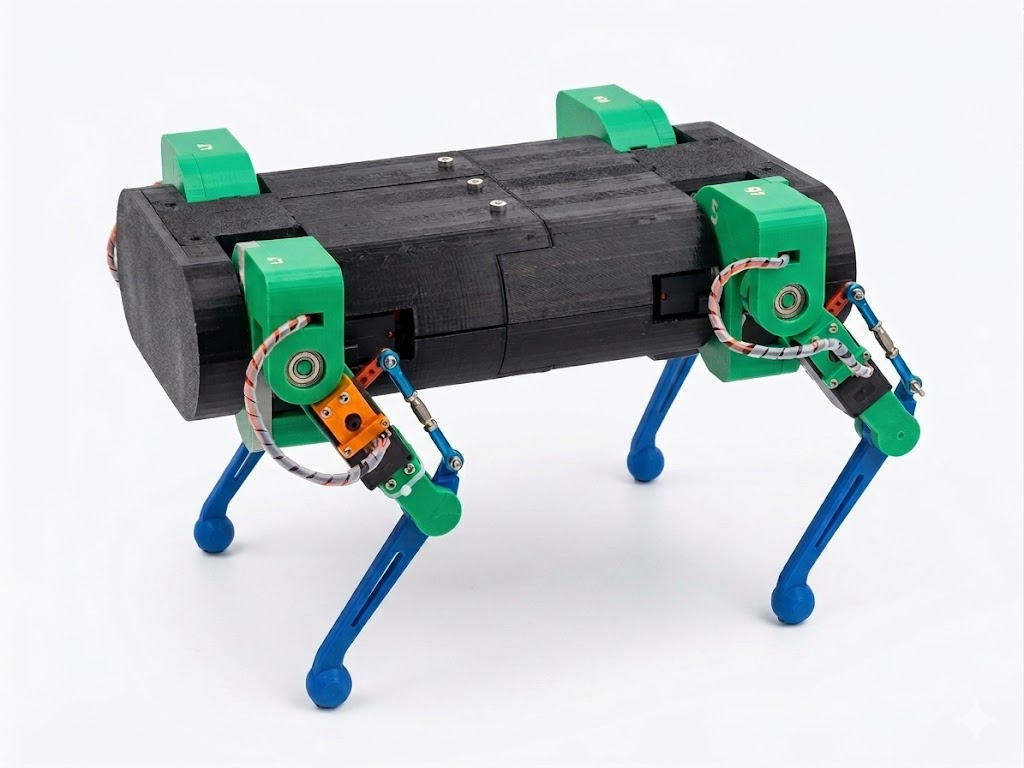
\includegraphics[width=\linewidth, height=0.6\textheight, keepaspectratio]{real_robot/quadrupedrobot.jpeg}
              \caption{Nguyên mẫu robot bốn chân hoàn thiện}
          \end{figure}
      \end{column}
  \end{columns}
\end{frame}
% --------------------------------------------------
\section{Thiết kế và thực hiện phần mềm}
% --------------------------------------------------

\begin{frame}{Tổng quan kiến trúc node}
  \begin{itemize}
      \item Kiến trúc phân tán rõ ràng giữa \texttt{gait\_generator} và \texttt{balance\_controller}.
      \item Dữ liệu vị trí và phản hồi IMU được đồng bộ nhanh chóng qua nền tảng DDS của ROS 2.
  \end{itemize}
  \vspace{-0.2cm}
  \begin{figure}
      \centering
      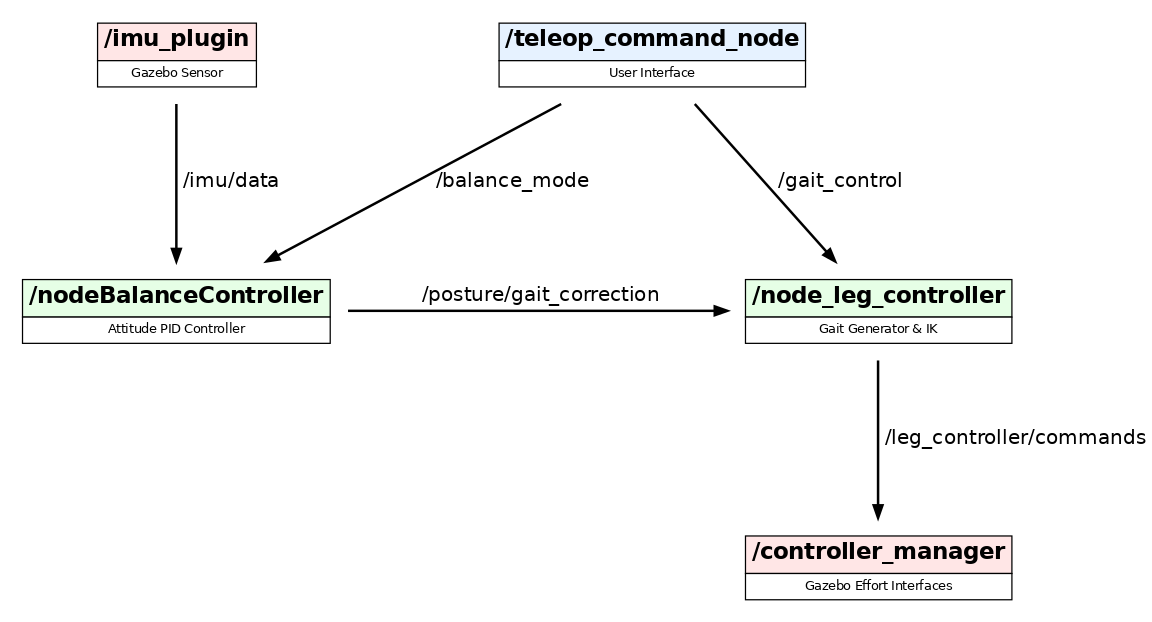
\includegraphics[width=0.9\linewidth, height=0.65\textheight, keepaspectratio]{architecture/simplified_ros2_graph.png}
      \caption{Mạng lưới các Node của ROS 2 (Môi trường mô phỏng)}
  \end{figure}
\end{frame}

\begin{frame}{Thiết kế thuật toán ổn định tư thế}
  \begin{columns}
      \begin{column}{0.4\textwidth}
          \begin{itemize}
              \item Tích hợp cảm biến BNO055 xử lý độ nghiêng Roll, Pitch.
              \item Xử lý nhiễu bằng lọc EMA và tạo vùng chết (Deadband) trước khi đưa vào bộ điều khiển.
              \item Làm mượt tín hiệu đầu ra (Low Pass Filter) bảo vệ cơ khí.
          \end{itemize}
      \end{column}
      \begin{column}{0.6\textwidth}
          \begin{figure}
              \centering
              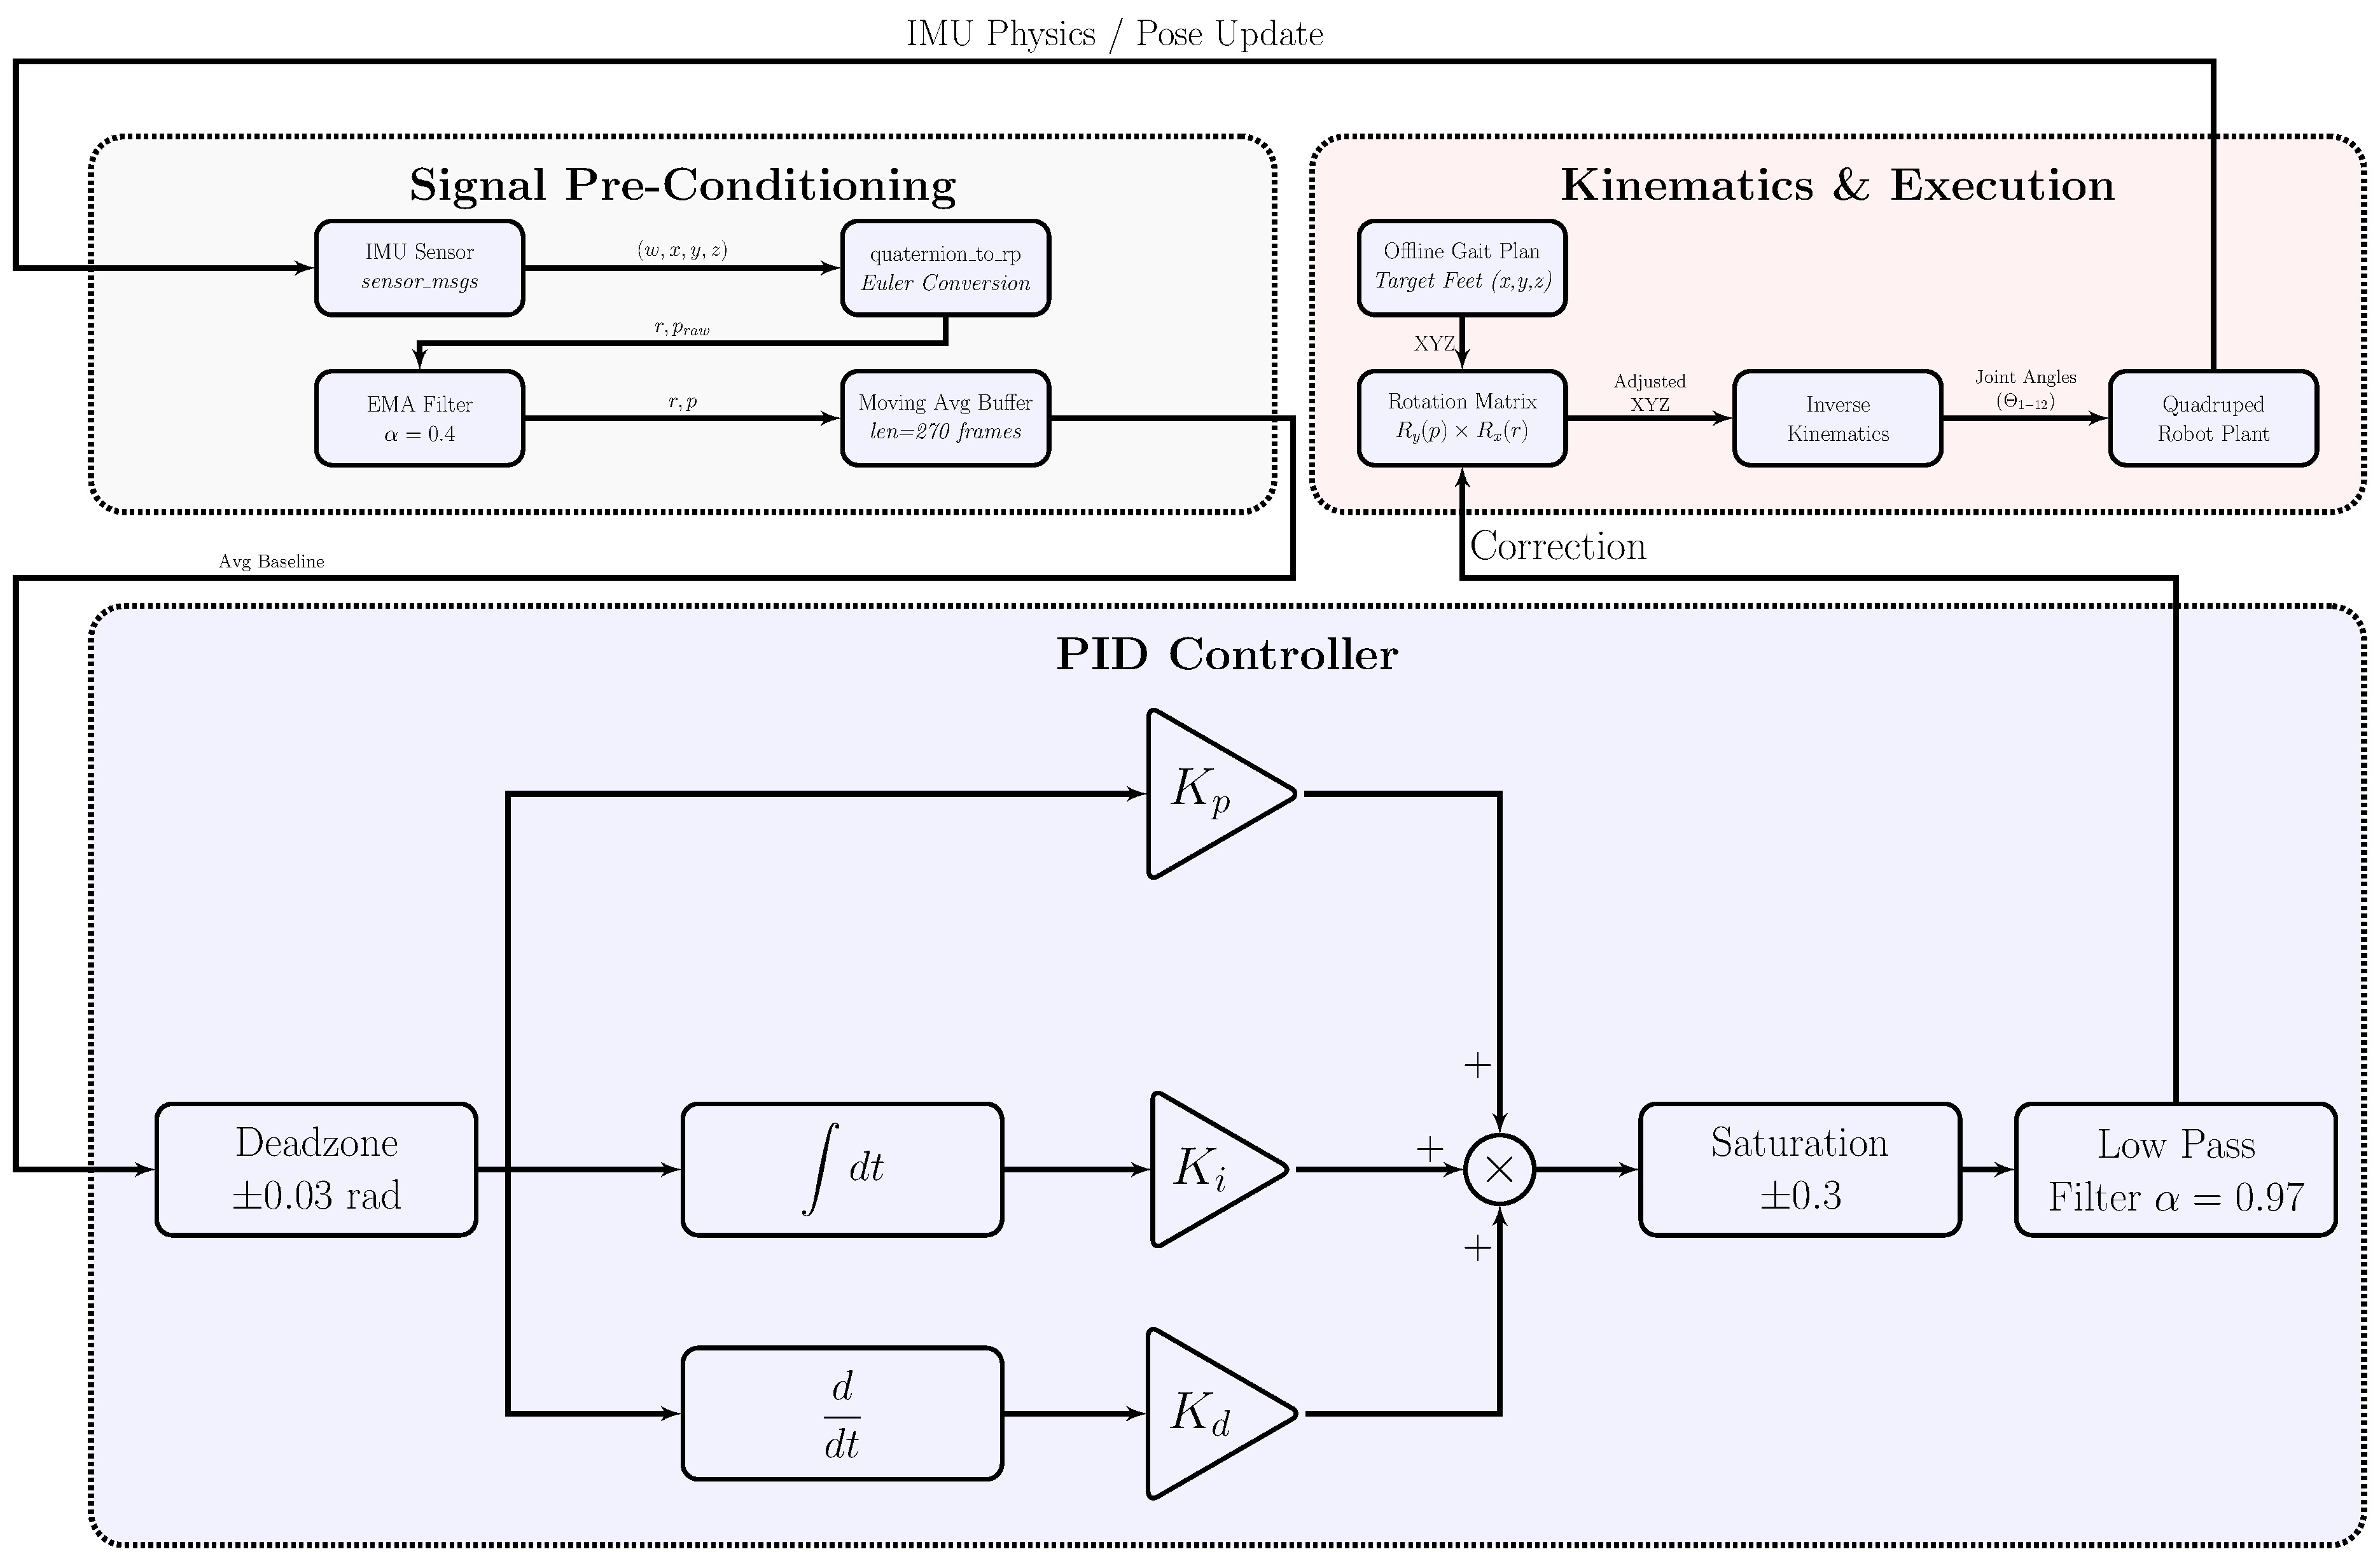
\includegraphics[width=\linewidth, height=0.7\textheight, keepaspectratio]{architecture/pid_architecture.pdf}
              \caption{Sơ đồ chuỗi xử lý tín hiệu PID 5 giai đoạn}
          \end{figure}
      \end{column}
  \end{columns}
\end{frame}

\begin{frame}{Hai chế độ bù trừ thăng bằng}
  \begin{columns}
      \begin{column}{0.5\textwidth}
          \textbf{Chế độ Tĩnh (HOME)}
          \begin{itemize}
              \item Khi robot đứng yên.
              \item Cộng trực tiếp tín hiệu (Roll, Pitch) vào phương trình IK ở không gian khớp.
              \item Phản hồi cực nhanh để dập tắt dao động.
          \end{itemize}
      \end{column}
      \begin{column}{0.5\textwidth}
          \textbf{Chế độ Động (GAIT)}
          \begin{itemize}
              \item Khi đang đi (chạy Trot).
              \item Tính bù thông qua ma trận xoay 3D (Cartesian) và chỉ tác dụng lên các chân chống (stance).
              \item Lọc Baseline trung bình trượt bỏ qua nhiễu bước chân.
          \end{itemize}
      \end{column}
  \end{columns}
\end{frame}

% --------------------------------------------------
\section{Kết quả và thảo luận}
% --------------------------------------------------

\begin{frame}{Đánh giá quy hoạch quỹ đạo offline}
  \begin{columns}
      \begin{column}{0.4\textwidth}
          \begin{itemize}
              \item Biên dạng vị trí trục $z$ sinh hình chữ D đặc trưng (D-shape).
              \item Vận tốc và gia tốc duy trì liên tục, bảo vệ vòng đời khớp nối.
          \end{itemize}
      \end{column}
      \begin{column}{0.6\textwidth}
          \begin{figure}
              \centering
              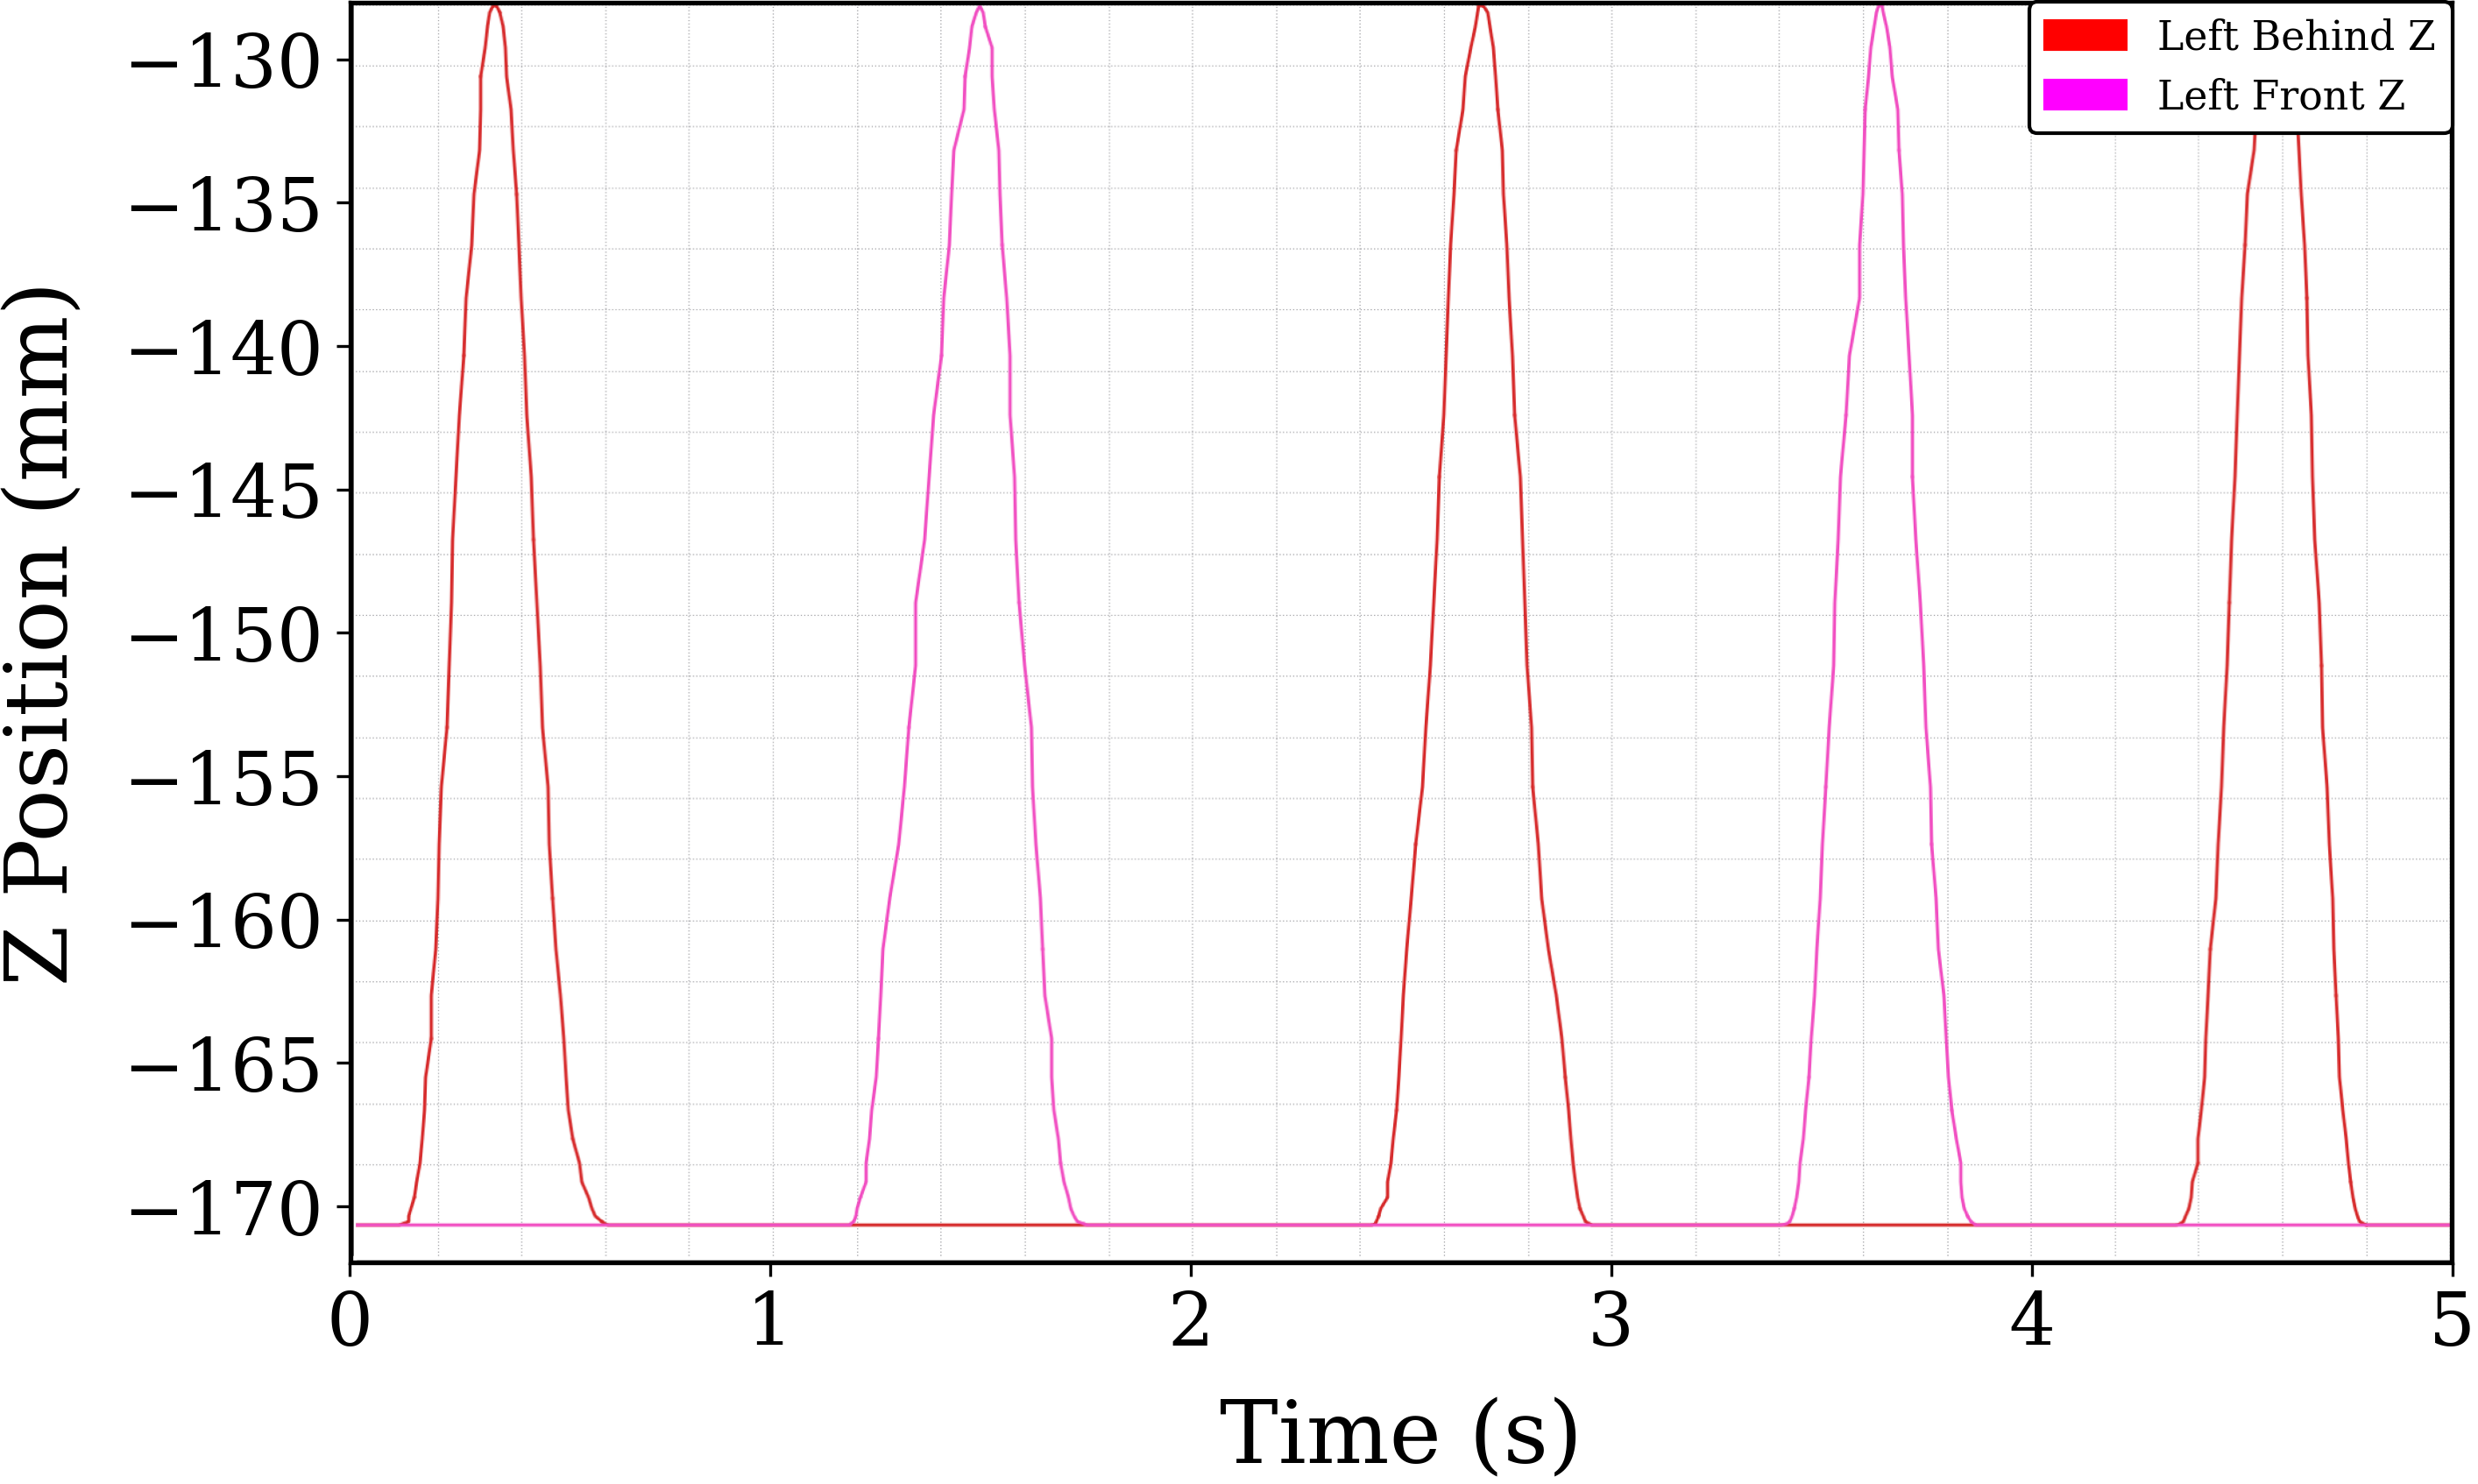
\includegraphics[width=\linewidth, height=0.7\textheight, keepaspectratio]{results/offline_traj_pos.png}
              \caption{Quỹ đạo hình chữ D lý thuyết}
          \end{figure}
      \end{column}
  \end{columns}
\end{frame}

\begin{frame}{Thực thi quỹ đạo trong Gazebo}
  \begin{columns}
      \begin{column}{0.4\textwidth}
          \begin{itemize}
              \item Bộ PD Torque của Gazebo điều khiển chân robot bám sát quỹ đạo offline.
              \item Minh chứng tính khả thi của thông số động lực học dưới ảnh hưởng trọng lực.
          \end{itemize}
      \end{column}
      \begin{column}{0.6\textwidth}
          \begin{figure}
              \centering
              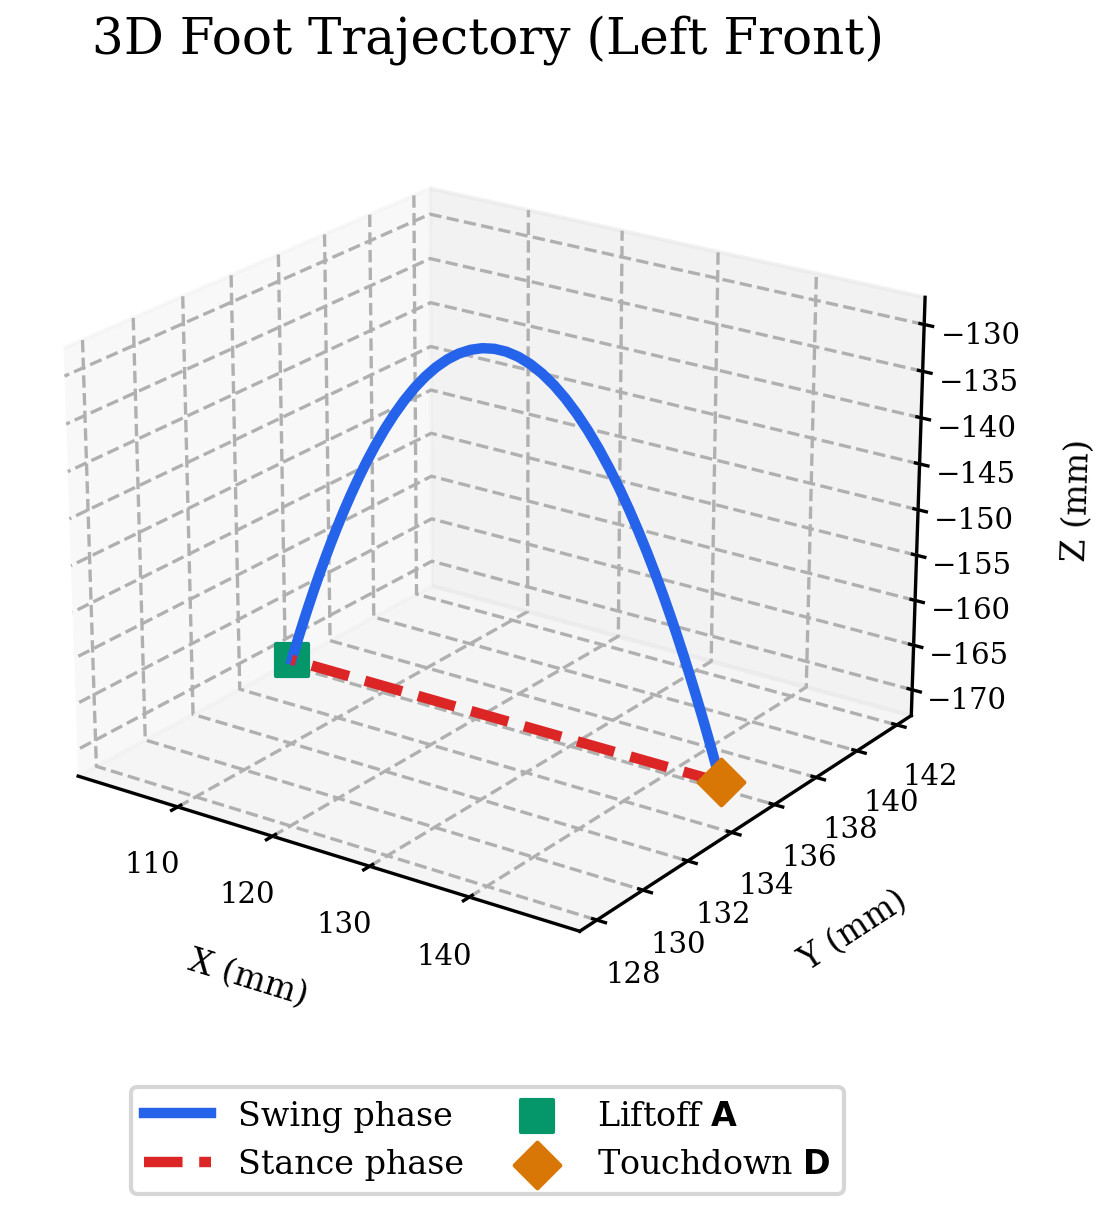
\includegraphics[width=0.7\linewidth, height=0.7\textheight, keepaspectratio]{gait_planner/gait_3d.png}
              \caption{Quỹ đạo thực tế ghi nhận trên Gazebo}
          \end{figure}
      \end{column}
  \end{columns}
\end{frame}

\begin{frame}{Đáp ứng ổn định tĩnh (HOME)}
  \begin{columns}
      \begin{column}{0.4\textwidth}
          \begin{itemize}
              \item Dập tắt xuất sắc dao động khi mặt phẳng rung lắc.
              \item Sự kiện Anti-windup ép tích phân không vượt ngưỡng, ngăn lật ngửa.
          \end{itemize}
      \end{column}
      \begin{column}{0.6\textwidth}
          \begin{figure}
              \centering
              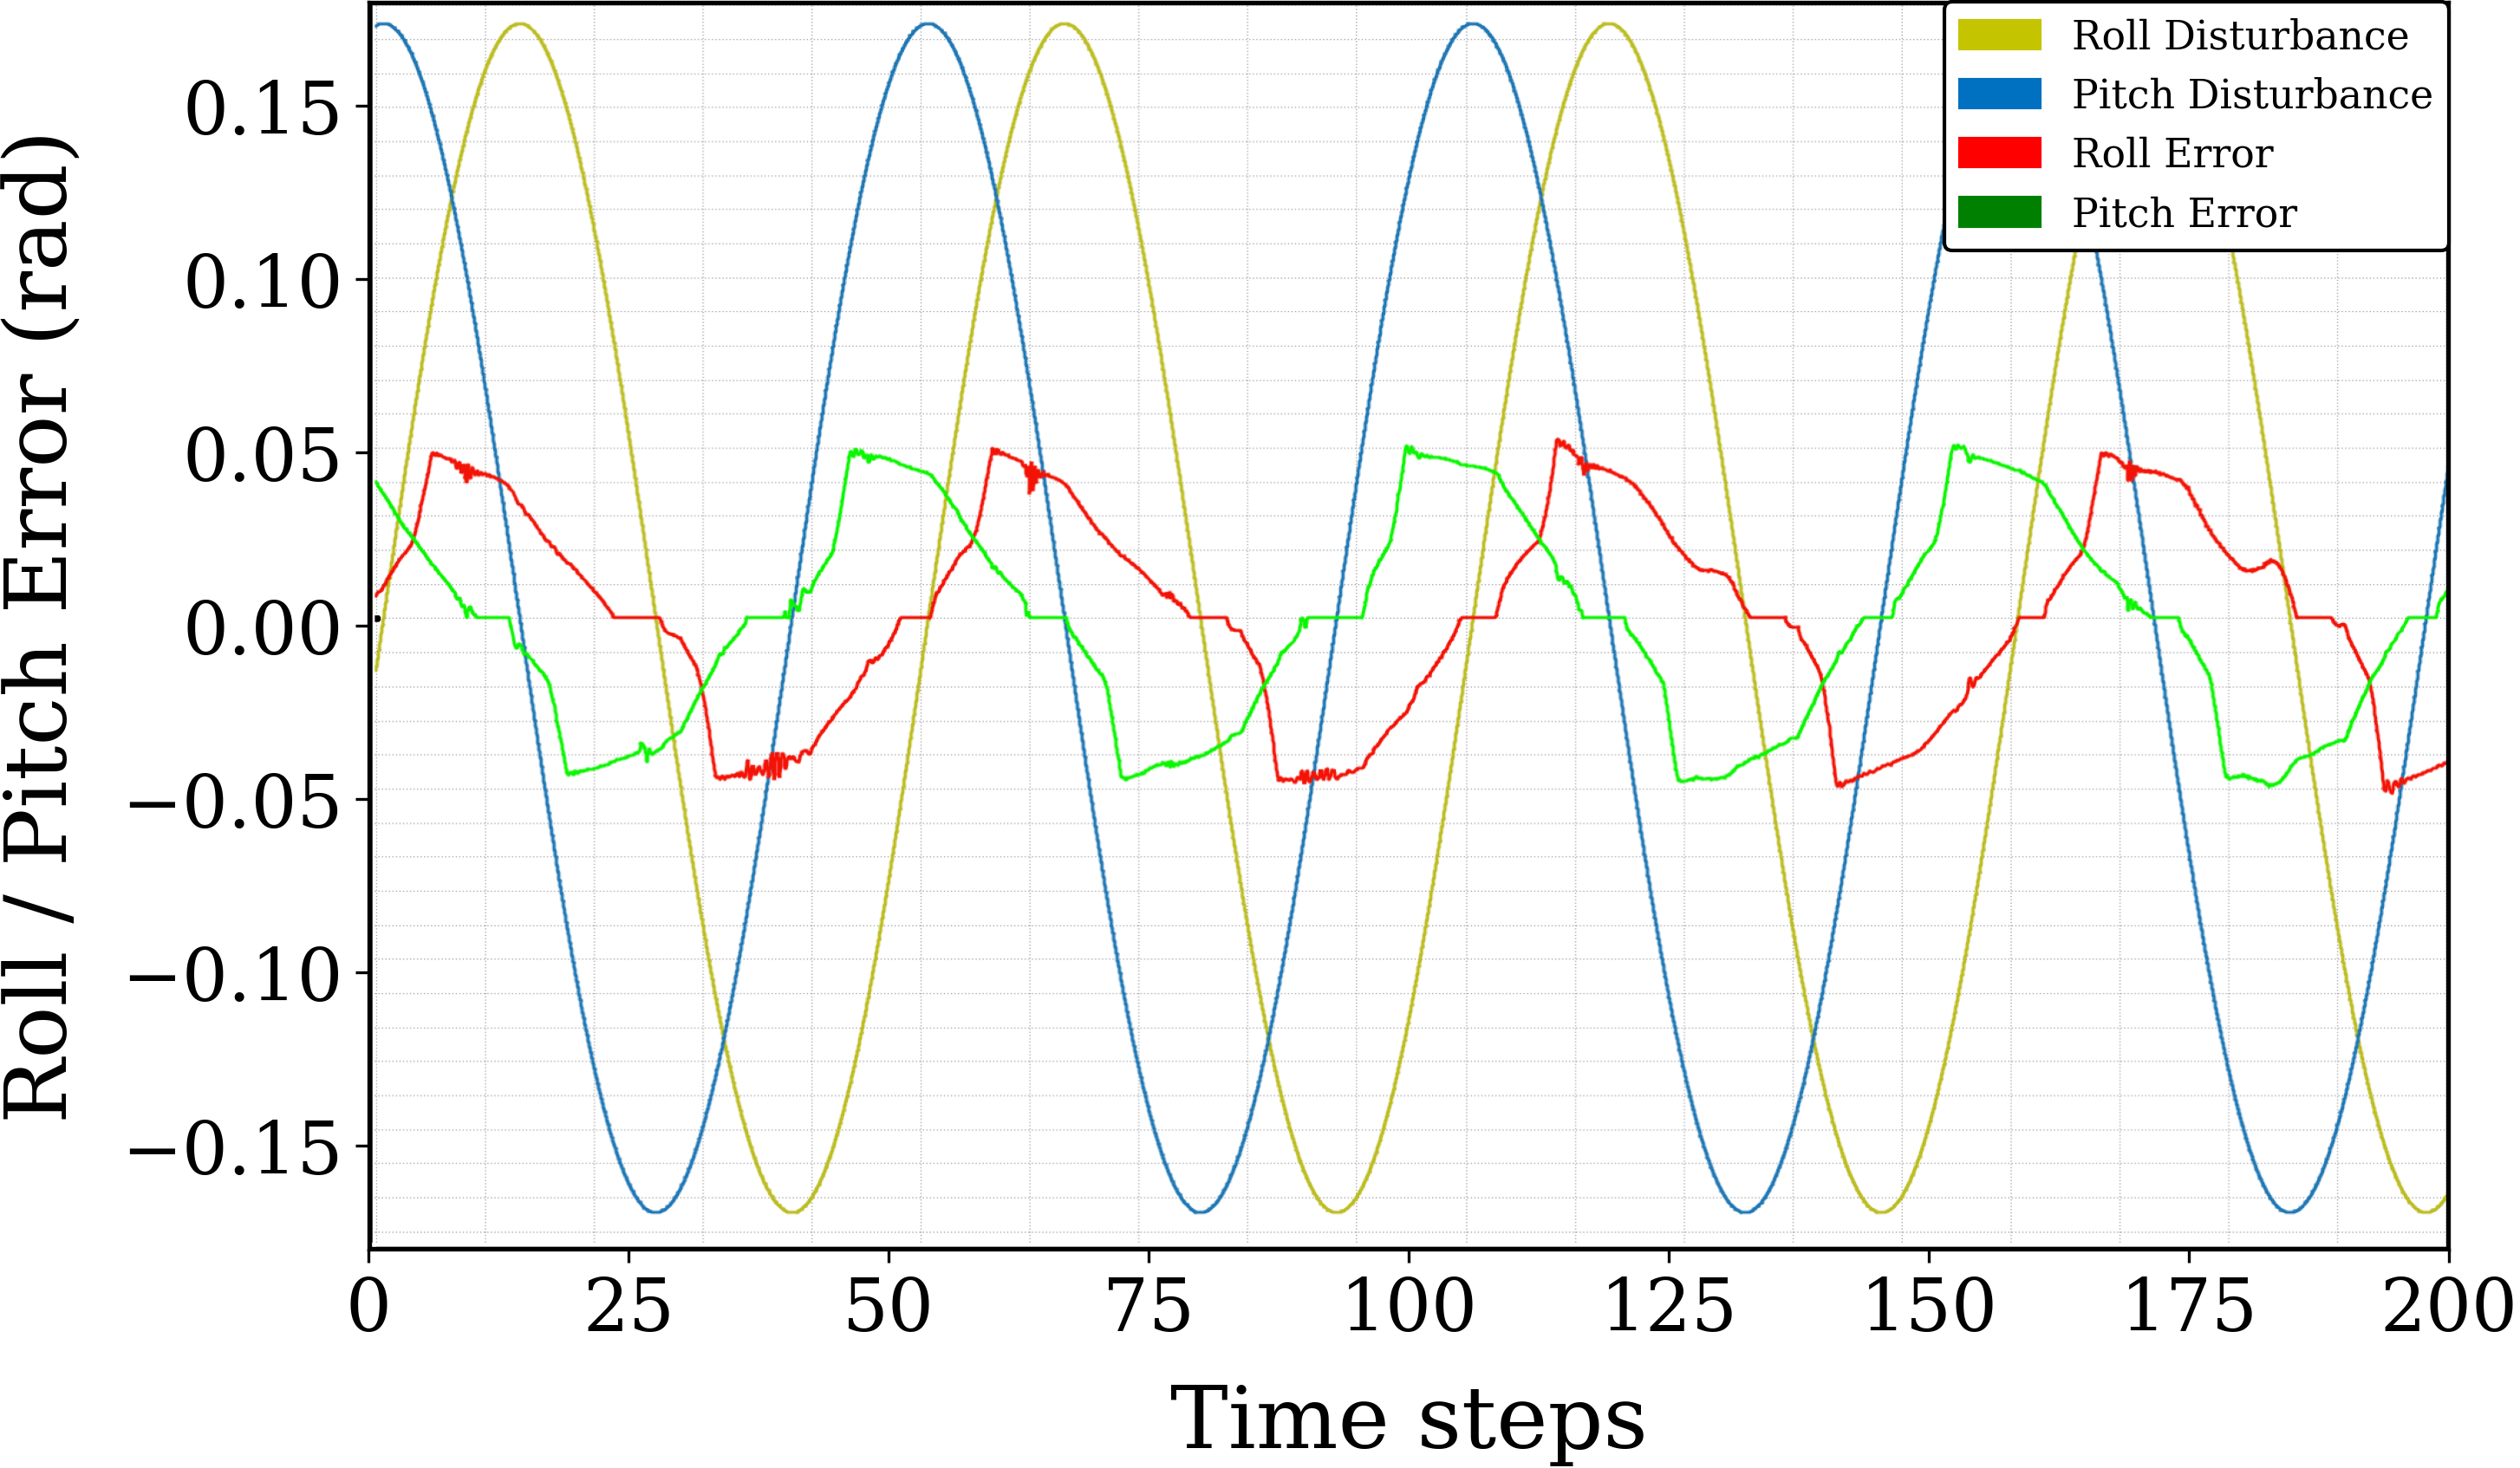
\includegraphics[width=\linewidth, height=0.7\textheight, keepaspectratio]{results/pid_error_home.png}
              \caption{Sai lệch Roll/Pitch khi chịu nhiễu mặt đất nghiêng}
          \end{figure}
      \end{column}
  \end{columns}
\end{frame}

\begin{frame}{Đáp ứng ổn định động (GAIT)}
  \begin{columns}
      \begin{column}{0.4\textwidth}
          \begin{itemize}
              \item Đảm bảo độ nghiêng luôn $\le \pm 0.08$ rad khi đi Trot.
              \item Cơ chế Reset tích phân triệt tiêu hiện tượng trôi dạt định hướng (attitude drift).
          \end{itemize}
      \end{column}
      \begin{column}{0.6\textwidth}
          \begin{figure}
              \centering
              
\includegraphics[width=\linewidth, height=0.7\textheight, keepaspectratio]{results/pid_error_gait.png}
              \caption{Thân robot được giữ cân bằng khi chạy Trot}
          \end{figure}
      \end{column}
  \end{columns}
\end{frame}

% --------------------------------------------------
\section{Kết luận và hướng phát triển}
% --------------------------------------------------

\begin{frame}{Đóng góp và Kết quả đạt được}
  \begin{enumerate}
      \item Hoàn thiện hệ thống "Sim-to-Real": Từ mô hình SolidWorks $\rightarrow$ ROS 2 / Gazebo $\rightarrow$ Robot thực 12 DOF.
      \item Triển khai quy hoạch quỹ đạo theo phương pháp nội suy đa thức bậc 5 mượt mà.
      \item Phát triển bộ cân bằng định hướng PID 5 giai đoạn, chia 2 mô hình toán học tĩnh/động chuyên biệt nhằm chống trôi lật.
  \end{enumerate}
  \vspace{0.3cm}
  \textbf{Hạn chế của phần cứng:}
  \begin{itemize}
      \item Trọng lượng thực tế nặng, động cơ ST3215 ở hai chân trước có dấu hiệu yếu tải tĩnh.
      \item Do đó thuật toán PID IMU động mới chứng minh hiệu quả cực cao ở khâu mô phỏng, và chưa được bật full trên robot thực.
  \end{itemize}
\end{frame}

\begin{frame}{Đề xuất Hướng phát triển}
  \begin{itemize}
      \item \textbf{Vật liệu:} Thay thế kết cấu in 3D bằng Carbon hoặc hợp kim để hạ tải trọng, tối ưu Pin LiPo xả cao.
      \item \textbf{Điều khiển cấp cao:} Nâng cấp điều khiển lực bằng MPC (Model Predictive Control) kết hợp điều khiển trở kháng (Impedance Control).
      \item \textbf{Học máy (AI):} Thay thế IK và cấu hình thủ công bằng Học Tăng Cường (Reinforcement Learning - RL) trên môi trường Isaac Gym.
      \item \textbf{Điều hướng không gian:} Bổ sung Depth Camera hướng tới bài toán SLAM tự động tránh vật cản.
  \end{itemize}
\end{frame}

\begin{frame}[plain]
    \begin{tikzpicture}[remember picture,overlay]
        % Corporate Minimalist Background (Navy Blue)
        \fill[hcmutblue] (current page.south west) rectangle (current page.north east);
        
        % Subtle massive watermark associated with project/organization
        \node[anchor=south east, opacity=0.06] at ([xshift=0.5cm, yshift=0cm]current page.south east) {
\includegraphics[height=0.7\textheight]{../presentation/reference/images/hcmut_logo_transparent.png}};

        % Main Thank you text (Centered, large)
        \node[anchor=south, text=white, font=\Huge\bfseries, scale=1.3] at ([yshift=0.8cm]current page.center) {XIN CẢM ƠN};
        \node[anchor=north, text=lightgray, font=\Large] at ([yshift=0.5cm]current page.center) {QUÝ THẦY CÔ TRONG HỘI ĐỒNG ĐÃ LẮNG NGHE};
        
        % Minimalist Red accent line separator
        \draw[hcmutred, line width=2pt] ([xshift=-4cm, yshift=-1.0cm]current page.center) -- ([xshift=4cm, yshift=-1.0cm]current page.center);
        
        % Group details
        \node[anchor=center, text=lightgray, font=\normalsize] at ([yshift=-3.3cm]current page.center) {ĐỒ ÁN TỐT NGHIỆP ĐẠI HỌC $\cdot$ ĐH BÁCH KHOA TP.HCM};
    \end{tikzpicture}
\end{frame}

\end{document}
